
\documentclass[final]{beamer}

\usepackage[scale=1.22]{beamerposter} % Use the beamerposter package for laying out the poster
\usepackage[spanish]{babel}

\usetheme{confposter} % Use the confposter theme supplied with this template

\setbeamercolor{block title}{fg=ngreen,bg=white} % Colors of the block titles
\setbeamercolor{block body}{fg=black,bg=white} % Colors of the body of blocks
\setbeamercolor{block alerted title}{fg=white,bg=dblue!70} % Colors of the highlighted block titles
\setbeamercolor{block alerted body}{fg=black,bg=dblue!10} % Colors of the body of highlighted blocks
% Many more colors are available for use in beamerthemeconfposter.sty

%-----------------------------------------------------------
% Define the column widths and overall poster size
% To set effective sepwid, onecolwid and twocolwid values, first choose how many columns you want and how much separation you want between columns
% In this template, the separation width chosen is 0.024 of the paper width and a 4-column layout
% onecolwid should therefore be (1-(# of columns+1)*sepwid)/# of columns e.g. (1-(4+1)*0.024)/4 = 0.22
% Set twocolwid to be (2*onecolwid)+sepwid = 0.464
% Set threecolwid to be (3*onecolwid)+2*sepwid = 0.708

\newlength{\sepwid}
\newlength{\onecolwid}
\newlength{\twocolwid}
\newlength{\threecolwid}
\setlength{\paperwidth}{48in} % A0 width: 46.8in
\setlength{\paperheight}{36in} % A0 height: 33.1in
\setlength{\sepwid}{0.024\paperwidth} % Separation width (white space) between columns
\setlength{\onecolwid}{0.22\paperwidth} % Width of one column
\setlength{\twocolwid}{0.464\paperwidth} % Width of two columns
\setlength{\threecolwid}{0.708\paperwidth} % Width of three columns
\setlength{\topmargin}{-0.5in} % Reduce the top margin size
%-----------------------------------------------------------

\usepackage{graphicx}  % Required for including images

\usepackage{booktabs} % Top and bottom rules for tables
\usepackage{multirow}
%----------------------------------------------------------------------------------------
%	TITLE SECTION 
%----------------------------------------------------------------------------------------

\title{Clasificación de texto basada en Transformers: comparación de representaciones y reducción de dimensiones} % Poster title

\author{Francisco Fernández Condado} % Author(s)

\institute{Universidad del País Vasco / Euskal Herriko Unibertsitatea} % Institution(s)

%----------------------------------------------------------------------------------------

\begin{document}

\addtobeamertemplate{block end}{}{\vspace*{2ex}} % White space under blocks
\addtobeamertemplate{block alerted end}{}{\vspace*{2ex}} % White space under highlighted (alert) blocks

\setlength{\belowcaptionskip}{2ex} % White space under figures
\setlength\belowdisplayshortskip{2ex} % White space under equations

\begin{frame}[t] % The whole poster is enclosed in one beamer frame

\begin{columns}[t] % The whole poster consists of three major columns, the second of which is split into two columns twice - the [t] option aligns each column's content to the top

\begin{column}{\sepwid}\end{column} % Empty spacer column

\begin{column}{\onecolwid} % The first column

%----------------------------------------------------------------------------------------
%	OBJECTIVES
%----------------------------------------------------------------------------------------

\begin{alertblock}{Objetivos}
\begin{itemize}
\item Objetivo: dado un texto corto, predecir la clase objetivo tratando de maximizar F-Score en la clase minoritaria.
\item Research questions: 
    \begin{description}
    \item[RQ1] ¿Qué modelo Transformer ofrece la mejor representación para estos datos?
    	\begin{enumerate}
    	\item RoBERTa
    	\item BERTweet
    	\end{enumerate}
    \item[RQ2] ¿Mejora los resultados aplicar una técnica de reducción de dimensionalidad?
        \begin{enumerate}
        	\item PCA
        	\item UMAP
        	\end{enumerate}
    \end{description}
\end{itemize}
\end{alertblock}

%----------------------------------------------------------------------------------------
%	QUICK REVISION
%----------------------------------------------------------------------------------------

\begin{block}{Tarea y datos}
% \textbf{Task}
\begin{itemize}
\item \textbf{Tarea:} clasificación binaria de textos con distribución de clases altamente desbalanceada.
\item \textbf{Distribución de clase RS:}
\begin{figure}
    \centering
    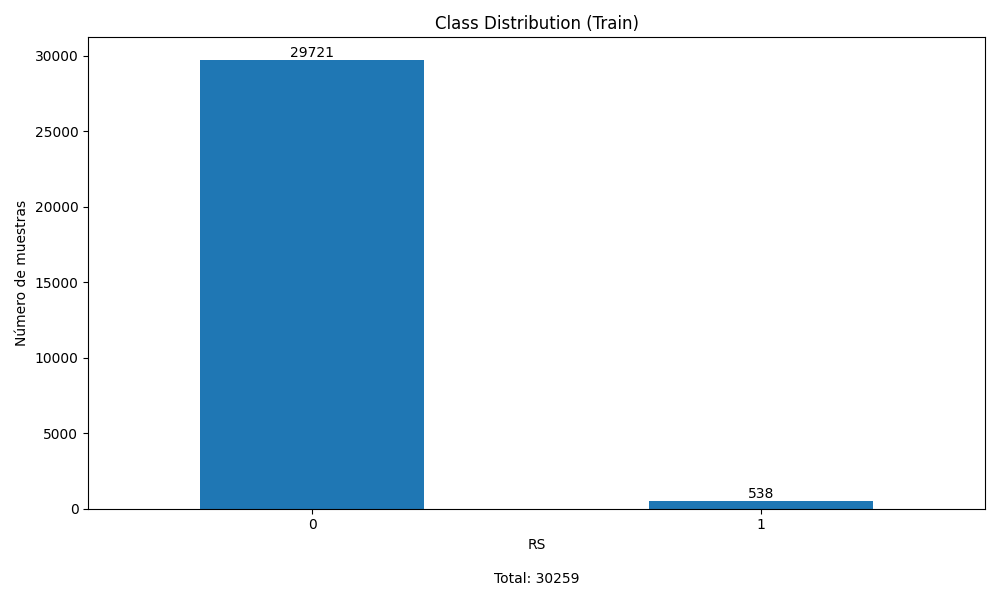
\includegraphics[width=0.9\linewidth]{class_distribution.png}
    \label{fig:class-distribution}
\end{figure}
\item \textbf{Longitud de los textos:}
\begin{figure}
    \centering
    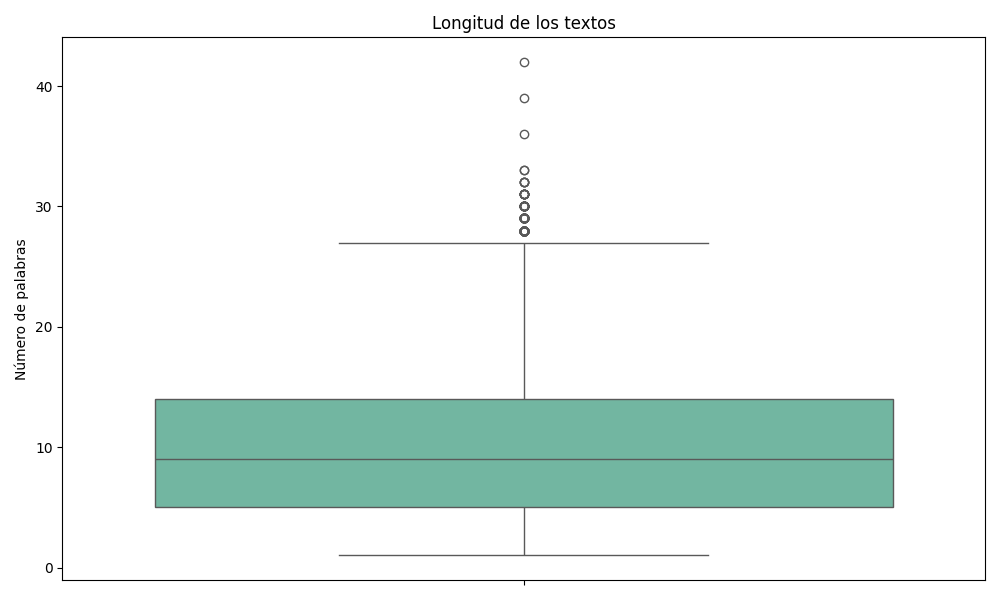
\includegraphics[width=0.9\linewidth]{doc_length_boxplot.png}
    \label{fig:class-length}
\end{figure}
\item \textbf{Pre-Proceso:} tokenización estándar y uso de embeddings basados en Transformers, descartando instancias inválidas.
\end{itemize}
% Describe the data before and after the data cleaning in a tabular way
% Data characterization: describe the features used to represent each text

\end{block}
\end{column} % End of the first column


%%%%%%%%%%%%%%%%%%%%%%%%%%%%%%%%%%%%%%%%
\begin{column}{\sepwid}\end{column} % Empty spacer column
    
    \begin{column}{\twocolwid} % Begin a column which is two columns wide (column 2)
                \begin{columns}[t,totalwidth=\twocolwid] % Split up the two columns wide column again
            %%%%%%%%%%        
            \begin{column}{\onecolwid} % The first column within column 2 (column 2.1)
            \begin{block}{Clasificador 1: RoBERTa}
            RoBERTa es un modelo de Transformer preentrenado de una forma muy similar a BERT, con mejoras interesantes en lo que respecta al impacto de grandes cantidades de hiperparámetros clave y el tamaño de los datos de entrenamiento.
            \end{block}
            \begin{block}{Algoritmo}
            Las pruebas han sido realizadas utilizando Random Forest aplicando SMOTE \cite{chawla2002smote} como técnica de Over-Sampling para reducir el desbalanceo.
            \end{block}
            \end{column} % End of column 2.1

            %%%%%%%%%%
            \begin{column}{\onecolwid} % The second column within column 2 (column 2.2)
            \begin{block}{Clasificador 2: BERTweet}
            BERTweet es otro modelo de Transformer entrenado de forma similar a BERT, pero en este caso optimizado para textos cortos. Se ha elegido por sus buenos resultados en pruebas experimentales \cite{guo-etal-2020-benchmarking} con datasets similares al utilizado, que se corresponden con textos de poca longitud con características típicas del lenguaje informal como el uso de emoticonos. Más adelante se aplicará con reducciones de dimensionalidad:
            \begin{itemize}
            % \item \url{http://www.cs.toronto.edu/~sjeblee/index.html}
            \item PCA
            \item UMAP
            \end{itemize}
            \end{block}
            \end{column} % End of column 2.2
            %%%%%%%%%%
        \end{columns} % End of the split of column 2
        %%%%%%%%%%
        
        % \begin{alertblock}{Implementation details}
        % \begin{itemize}
        % \item 
        % \item Parameters chosen for each classification. Fine-tuning strategy
        % \end{itemize}
        % \end{alertblock} 
        %%%%%%%%%%
        \begin{columns}[t,totalwidth=\twocolwid] % Split up the two columns wide column again
            \begin{column}{\twocolwid}
            \begin{block}{Resultados experimentales: RQ1}
            Para comparar el mejor clasificador, se han realizado pruebas experimentales usando el mismo conjunto de datos, aplicando SMOTE con los mismos parámetros y empleando las distintas vectorizaciones que propone tanto un modelo como otro.
            
                %%%%%%%%%%        
                \begin{column}{\onecolwid} % The first column within column 2 (column 2.1)
                % \begin{block}{Results: }
                
                \begin{figure}
                    \centering
                    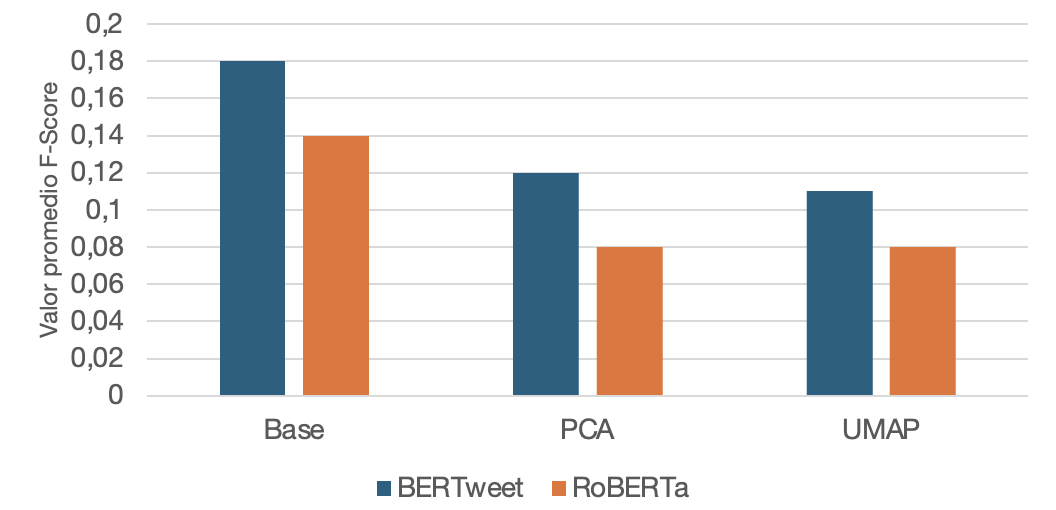
\includegraphics[width=1\linewidth]{bertweet-roberta.png}
                    \caption{Valores promedios de F-Score para la clase minoritaria usando BERTweet y RoBERTa}
                    \label{fig:bertweet-roberta}
                \end{figure}
                \begin{itemize}
                \item \textbf{Configuraciones:} 
                \begin{itemize}
                    \item RoBERTa: Fine-tuning con learning rate $1\times10^{-5}$ y batch size 16.
                    \item BERTweet: Fine-tuning con learning rate $3\times10^{-5}$ y batch size 32.
                    \item 5 iteraciones por cada prueba
                \end{itemize}
                \item Los resultados muestran mejores valores para F-Score, Accuracy y Recall utilizando BERTweet frente a RoBERTa, independientemente de la reducción de dimensionalidad.
            \end{itemize}
                % \end{block}
                \end{column} % End of column 2.1
                %%%%%%%%%%
                \begin{column}{\onecolwid} % The second column within column 2 (column 2.2)
                % \begin{block}{Experimental results}
                \begin{table}[ht]
                \centering
                \begin{tabular}{|l|l|c|}
                \hline
                \textbf{Clasificador} & \textbf{Método} & \textbf{Resultados (mean)} \\ \hline
                BERTweet & Base  & Accuracy: 0.96 \\ 
                         &       & F1-Score: 0.18 \\ 
                         &       & Recall: 0.21 \\ \hline
                BERTweet & PCA   & Accuracy: 0.94 \\ 
                         &       & F1-Score: 0.12 \\ 
                         &       & Recall: 0.22 \\ \hline
                BERTweet & UMAP  & Accuracy: 0.92 \\ 
                         &       & F1-Score: 0.11 \\ 
                         &       & Recall: 0.25 \\ \hline
                RoBERTa  & Base  & Accuracy: 0.96 \\ 
                         &       & F1-Score: 0.14 \\ 
                         &       & Recall: 0.16 \\ \hline
                RoBERTa  & PCA   & Accuracy: 0.93 \\ 
                         &       & F1-Score: 0.08 \\ 
                         &       & Recall: 0.17 \\ \hline
                RoBERTa  & UMAP  & Accuracy: 0.97 \\ 
                         &       & F1-Score: 0.08 \\ 
                         &       & Recall: 0.08 \\ \hline
                \end{tabular}
                \caption{Resultados medios de las experimentaciones. BERTweet ofrece una mayor precisión y exhaustividad en todas las pruebas realizadas}
                \label{tab:summary}
            \end{table}
                \end{column} % End of column 2.2
                %%%%%%%%%%
                
            \end{block}
            \end{column}
        \end{columns} % End of the split of column 2
\end{column} % End of the second column
%%%%%%%%%%%%%%%%%%%%%%%%%%%%%%%%%%%%%%%%



\begin{column}{\sepwid}\end{column} % Empty spacer column
\begin{column}{\onecolwid} % The third column
%----------------------------------------------------------------------------------------
%	CONCLUSION
%----------------------------------------------------------------------------------------

\begin{block}{Resultados experimentales: RQ2}
% Show the experiments carried out to make a decision about the characterization

    \begin{figure}
        \centering
        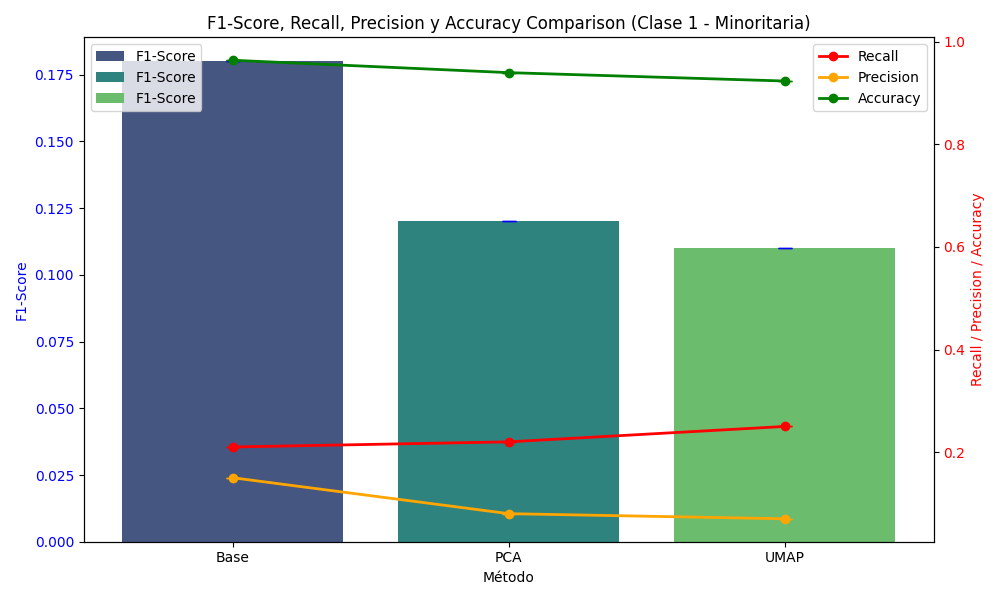
\includegraphics[width=1\linewidth]{f1_recall_precision_comparison.png}
        \caption{Comparativa de métricas usando BERTweet}
        \label{fig:metricas}
    \end{figure}
    
    \begin{itemize}
    \item Los resultados muestran una mayor precisión al no aplicar reducción de dimensionalidad.
    \item UMAP mejora ligeramente la exhaustividad.
    \item RF da mejor resultado con más parámetros.
    \end{itemize}
\end{block}




%----------------------------------------------------------------------------------------
%	ACKNOWLEDGEMENTS
%----------------------------------------------------------------------------------------

%\setbeamercolor{block title}{fg=red,bg=white} % Change the block title color
% \begin{block}{Glossary}
% \begin{table}
% \vspace{2ex}
% \begin{tabular}{l l l l}
% \toprule
% \textbf{verb} & \textbf{noun} & \textbf{meaning}\\
% \midrule
% add & addition & $+$ \\
% subtract & subtraction & $-$ \\
% multiply & multiplication & $\cdot$ \\
% divide & division & $\div$ \\
% solve & solution & getting answer \\
% substitute & substitution & $t=x^2$ \\
% \bottomrule
% \end{tabular}
% \caption{Word Formation}
% \end{table}


% \end{block}

\setbeamercolor{block alerted title}{fg=black,bg=norange} % Change the alert block title colors
\setbeamercolor{block alerted body}{fg=black,bg=white} % Change the alert block body colors

\begin{alertblock}{Conclusiones y trabajo futuro} 
 
    \begin{itemize}
    \item Resumen: se han explorado \alert{2 clasificadores + 2 análisis} para ver cuál ofrece mejores resultados.
    \item Para estos datos, la mejor opción en cuanto a precisión es utilizar BERTweet sin reducción, UMAP mejora tiempos.
    \item Convendría realizar las mismas pruebas con otros datos. Probablemente en textos largos no se obtengan los mismos resultados, así como probar otras técnicas y embeddings.
    \end{itemize}

\end{alertblock}

% ---------------------------------------------
\setbeamercolor{block title}{fg=dblue!70,bg=white} % Change the block title color
\begin{block}{\small Bibliografía}
\footnotesize
\bibliographystyle{apalike}
\bibliography{myBibliography}
\end{block}



%----------------------------------------------------------------------------------------

\end{column} % End of the third column

\end{columns} % End of all the columns in the poster

\end{frame} % End of the enclosing frame

\end{document}
